\section{Musterauswertung}

\subsection*{Diodenflussspannung}
Die Diodenflussspannung $U_{D}$ ergibt sich aus dem Schnittpunkt des linearen Teils der Kennlinie mit der x-Achse. Die Messwerte für die Diode sind in Abbildung \ref{diode} aufgetragen, die Messwerte für die unbeleuchtete Solarzelle in Abb. \ref{solar}. Beide Graphen enthalten einen linearen Fit\footnote{$\chi^{2}$-Fit mit gnuplot.} zur Bestimmung der Diodenflussspannung. Die Fehler der Geradenparameter aus dem Fit wurden direkt mit Gaußscher Fehlerfortpflanzung benutzt um die Fehler der x-Achsen Schnittpunkte zu berechnen. Damit ergibt sich für die Diode $U_{D,D}=0.7\pm 0.2$\;V und für die Solarzelle $U_{D,S}=0.5\pm 0.1$\;V.
\begin{figure}
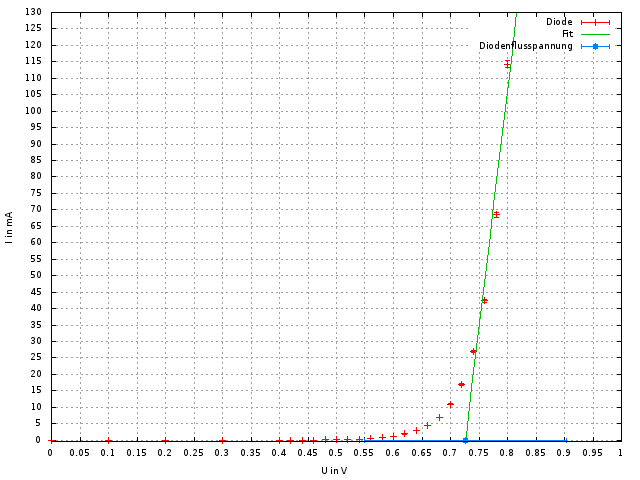
\includegraphics[scale=0.6]{Auswertung/Diode.png}
\caption{Kennlinie der Diode mit auf 1\% geschätztem Fehler, linearem Fit und daraus berechneter Diodenflusspannung}
\label{diode}
\end{figure}
\begin{figure}
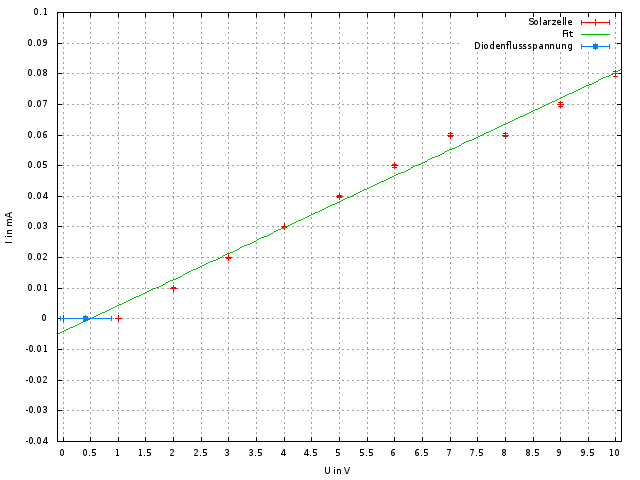
\includegraphics[scale=0.6]{Auswertung/Solar.png}
\caption{Kennlinie der unbeleuchteten Solarzelle mit auf 1\% geschätztem Fehler, linearem Fit und daraus berechneter Diodenflusspannung}
\label{solar}
\end{figure}

\subsection*{Kurzschlusstrom und Leerlaufspannung}
Die Kennlinien der beleuchteten Solarzelle für verschiedene, oder ohne Farbfilter sind in Abb. \ref{blau},\ \ref{gelb},\ \ref{gruen} und \ref{unge} aufgetragen, wobei die systematischen Fehler nach Versuchsanleitung auf 1\% geschätzt wurden. Aus Stromstärke $I(U=0)$ ergibt sich der Kurzschlusstrom $I_{k}$ für die verschiedenen Bestrahlungen. Analog lässt sich die Leerlaufspannung $U_{L}=U(I=0)$ über lineare Extrapolation der Werte für große $U$ bestimmen. Der Fehler des Kurzschlusstroms kann über den Fehler für den gemessenen Wert bestimmt werden und der Fehler für die Leerlaufspannung nur grob geschätzt werden, da die lineare Extrapolation das tatsächliche Verhalten nicht korrekt widerspiegelt. Die somit erhaltenen Werte mit Fehler sind in Tabelle \ref{werte} aufgelistet.\\
\begin{table}
\begin{center}
\begin{tabular}{|c|c|c|}
&$I_{k}$ in mA&$U_{L}$ in V\\
\hline
ungefiltert&$5.4\pm 0.1$ &$12.2 \pm 0.4$ \\
\hline
blau&$2.55\pm 0.05$ &$7.6\pm 0.2$\\
\hline
grün&$2.49\pm 0.05$ & $7.5 \pm 0.2$\\
\hline 
gelb&$3.94\pm 0.07$ & $9.4\pm 0.3$\\
\hline
\end{tabular}
\caption{Kurzschlussstrom und Leerlaufspannung der Solarzelle.\label{werte}}
\end{center}
\end{table}
\begin{figure}
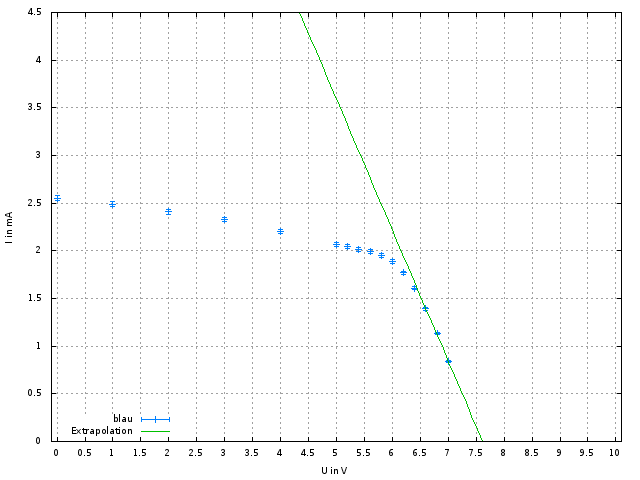
\includegraphics[scale=0.6]{Auswertung/blau.png}
\caption{Kennlinie der mit blauem Licht beleuchteten Solarzelle mit linearer Extrapolation zu U=0.\label{blau}}
\end{figure}
\begin{figure}
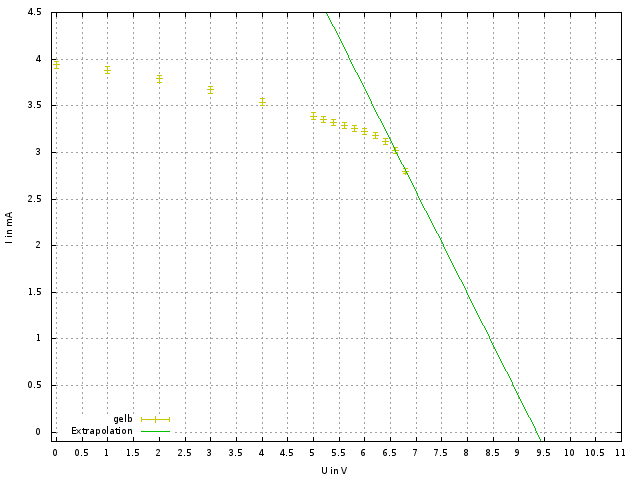
\includegraphics[scale=0.6]{Auswertung/gelb.png}
\caption{Kennlinie der mit gelbem Licht beleuchteten Solarzelle mit linearer Extrapolation zu U=0.\label{gelb}}
\end{figure}\begin{figure}
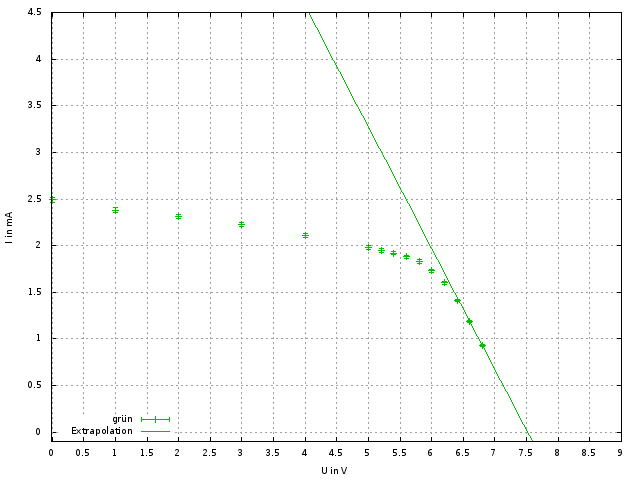
\includegraphics[scale=0.6]{Auswertung/gruen.png}
\caption{Kennlinie der mit grünem Licht beleuchteten Solarzelle mit linearer Extrapolation zu U=0.\label{gruen}}
\end{figure}\begin{figure}
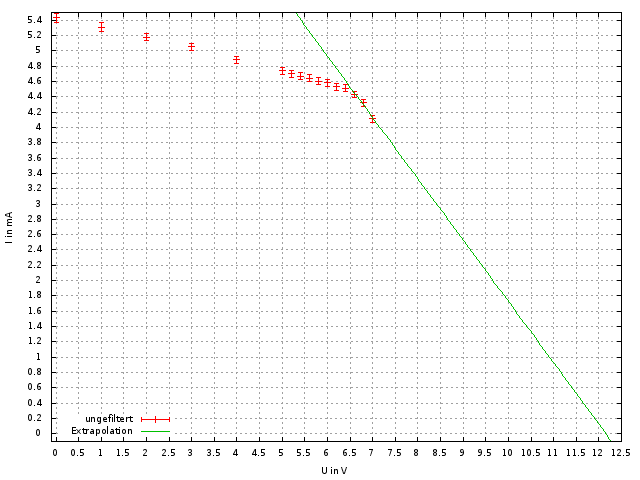
\includegraphics[scale=0.6]{Auswertung/ungefiltert.png}
\caption{Kennlinie der mit weißem Licht beleuchteten Solarzelle mit linearer Extrapolation zu U=0.\label{unge}}
\end{figure}


\subsection*{Maximal Power Point}
Der Maximal Power Point der Solarzelle lässt sich aus dem Maximum der $P(U)$-Kurve bestimmen. Diese ist für die verschiedenen Farbfilter in Abb. \ref{power} aufgetragen. Die maximal erreichte Leistung für jede Farbe mit den entsprechenden Spannungs- und Stromwerten sind in Tabelle \ref{mpp} aufgelistet. Die Fehler der Leistung sind über gaußsche Fehlerfortpflanzung bestimmt.
\begin{table}
\begin{center}
\begin{tabular}{|c|c|c|c|}
&$P_{max}$ in mW&$I_{max}$ in mA&$U_{max}$ in V\\
\hline
blau& $11.3\pm 0.2$ &1.89&6\\
\hline
grün& $10.6\pm 0.2$ &1.83&5.8\\
\hline
gelb& $19.97\pm 0.3$ &3.12&6.4\\
\hline
weiß& $29.4\pm 0.4$ &4.32 &6.8\\
\hline
\end{tabular}
\end{center}
\caption{Leistungsmaxima und die zugehörigen Spannungs- und Stromwerte.\label{mpp}}
\end{table}
\begin{figure}
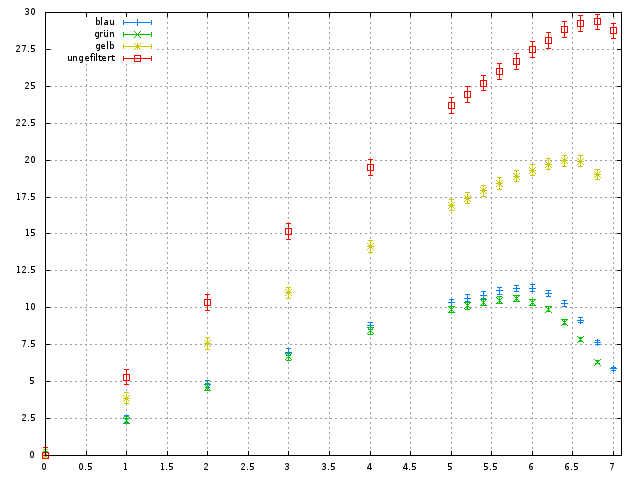
\includegraphics[scale=0.6]{Auswertung/power.png}
\caption{Leistung der Solarzelle für verschiedene Bestrahlungsfarben in Abhängigkeit der Spannung.\label{power}}
\end{figure}

\subsection*{Spektrale Empfindlichkeit der Solarzelle}
Die Empfindlichkeit der Zelle wird untersucht, indem das Verhältnis der Empfindlichkeit bei Einfall von grünen bzw. gelbem Licht ausgerechnet wird. Es lässt sich aus folgender Gleichung bestimmen, da Leistung der Lampe mit gelbem Filter um 10\% größer ist als mit grünem Farbfilter:
\begin{align*}
\frac{S_{gelb}}{S_{gruen}}&=\frac{I_{k}(gelb)}{1.1\cdot I_{k}(gruen)},\\
\frac{S_{gelb}}{S_{gruen}}&=1.44\pm 0.04.\\
\end{align*}
Aus der in der im Diagramm aus der Anleitung gegebenen Empfindlichkeiten $S_{gelb}\approx 0.34$ und $S_{gruen}\approx 0.23$ ergibt sich ein Vergleichswert von $\frac{S_{gelb}}{S_{gruen}}\approx 1.48$.
 \end{document}